\newpage
\chapter{Results \& Discussion}

    \section{CNN Model}
    \noindent
    The model developed for the deployment has the following parameters at each layer:
    \begin{figure}[H]
        \centering
        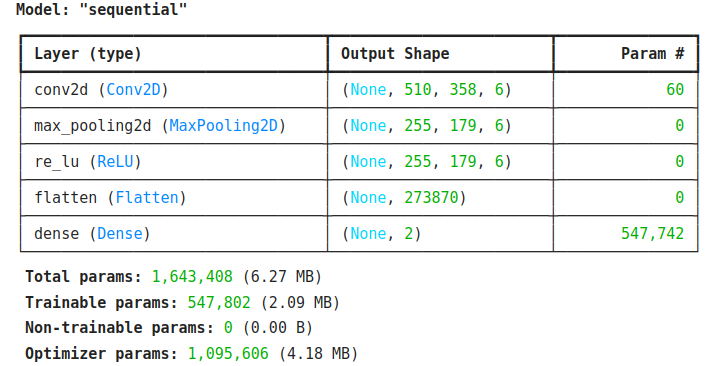
\includegraphics[width=1\linewidth]{images/modelSummary.png}
        \caption{Model Summary}
        \label{fig:enter-label}
    \end{figure}
    The following are the hyperparameters:
    \begin{enumerate}
        \item Number of epochs 15
        \item Activation function ReLU for the convolution layer and Softmax for final probabilities
    \end{enumerate}

    \noindent
    A validation accuracy of 92.22\% is obtained when tested on a validation dataset. The following figures show the Training and Validation accuracy plots and the confusion matrix. It must be noted that all benign cases are accurately predicted. This is specific to the validation dataset for some other set of datasets, this may not be the case.

    \begin{figure}[H]
        \centering
        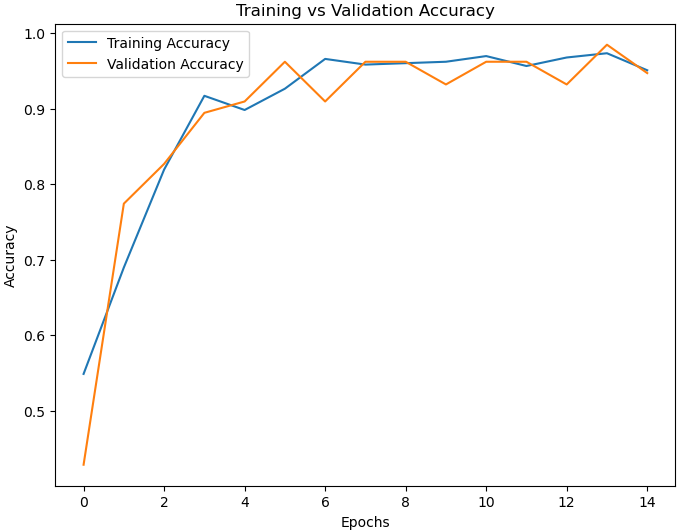
\includegraphics[width=1\linewidth]{images/trainValAcc.png}
        \caption{Train and Validation Accuracy Plot}
        \label{fig:enter-label}
    \end{figure}

    \noindent
    Some of the classification model parameters have been shown below, as per the reports generated in Python from Jupyter:

    \begin{figure}[H]
        \centering
        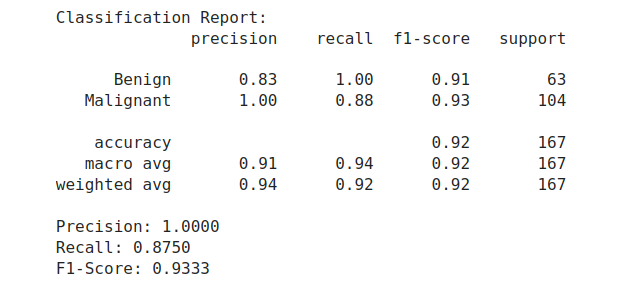
\includegraphics[width=1\linewidth]{images/classificationReport.png}
        \caption{Classification Report for the CNN model}
        \label{fig:enter-label}
    \end{figure}

    \begin{figure}[H]
        \centering
        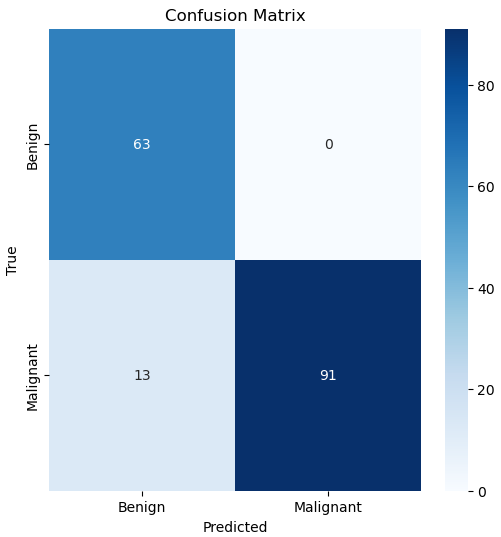
\includegraphics[width=0.75\linewidth]{images/conf_matrix.png}
        \caption{Confusion Matrix evaluated on Validation dataset}
        \label{fig:enter-label}
    \end{figure}
    
    \section{FPGA Experimental Results Analysis}
    \noindent
    The final convolution and max pool logic are evaluated on the hardware, and it is observed and verified that the desired appropriate feature maps are being generated.
    The entire design is implemented on the PYNQ-Z2 FPGA, which belongs to the Xilinx (now AMD) ZYNQ 7000 SoC series. The entire design was evaluated well for the timing performance at 100MHz, but while the final block level design, since the Vivado placer is not well optimized, it led to some routing congestion, and as a result, a slack of 0.105ns was observed, hence the final design works on a frequency slightly less than 100MHz. The table \ref{tab:onchip-resources} shows the resource utilisation report for the design implemented on the PL fabric.

    \begin{table}[h!]
    \centering
    \begin{tabular}{|l|c|c|c|}
        \hline
        \textbf{On-chip resources} & \textbf{Number of resources} & \textbf{Occupied resources} & \textbf{Utilization} \\
        \hline
        LUTs         & 53,200    & 9,529     & 17.9\%   \\
        Flip-Flops   & 106,400   & 7,122     & 6.69\%   \\
        BRAM         & 140       & 128.5     & 91.79\%  \\
        DSP Slices   & 220       & 9         & 4.09\%   \\
        \hline
    \end{tabular}
    \caption{FPGA On-Chip Resource Utilisation}
    \label{tab:onchip-resources}
    \end{table}

    \noindent

    \[
    \text{TPS} = \frac{\text{BITS}}{T}
    \]
    Some performance metrics are discussed in the previous work by Li Li et. al [1]. \par \noindent
    The above formula, TPS, is the throughput, BITS is the number of bits operated in time T. Considering a clock frequency of 100MHz, the proposed system throughput is,

    \[
    \text{TPS} = 360 \times 512 \times 16 \times 100\,\text{MHz} = 294.912\,\text{Gbit/s}
    \]

    \[
    P = \frac{\text{Opt}}{\text{Clk\_num}}
    \]
    Where P stands for computing performance, Clk\_num is the number of required clock cycles to complete operations, and Opt is the number of operations.
    
    \begin{table}[H]
    \centering
    \begin{tabular}{|l|c|}
        \hline
        \textbf{Layer} & \textbf{Number of Operations} \\
        \hline
        Convolution & 360x512x9 \\
        Maxpool     & 358x510x3 \\
        Total       & 2206620   \\
        \hline
    \end{tabular}
    \caption{Layer and Number of Operations}
    \label{tab:layer_operations}
    \end{table}

    \noindent
    As per the simulation results, it is observed that the output feature map is obtained after 1855005 ns and starts at 26175 ns. So the total number of clock cycles required for the operation is (1855005-26175)/10 = 182883 cycles. Thus, the computing performance is 12.066 GOP/s, the power consumption is 1.484W, and the energy efficiency is 8.13 GOP/(s.W).

    \section{Experimental Setup}
    \noindent
    The figure \ref{fig:expSetup} shows the experimental setup, as shown in the image, the PYNQ-Z2 board is connected to the PC through Microusb Port, which is also used as a  UART port and employs a USB to UART bridge for UART interface. The Red LED indicates power status, and the  Green LED is the DONE bit, which is HIGH as seen in the setup.
    
    \begin{figure}[H]
        \centering
        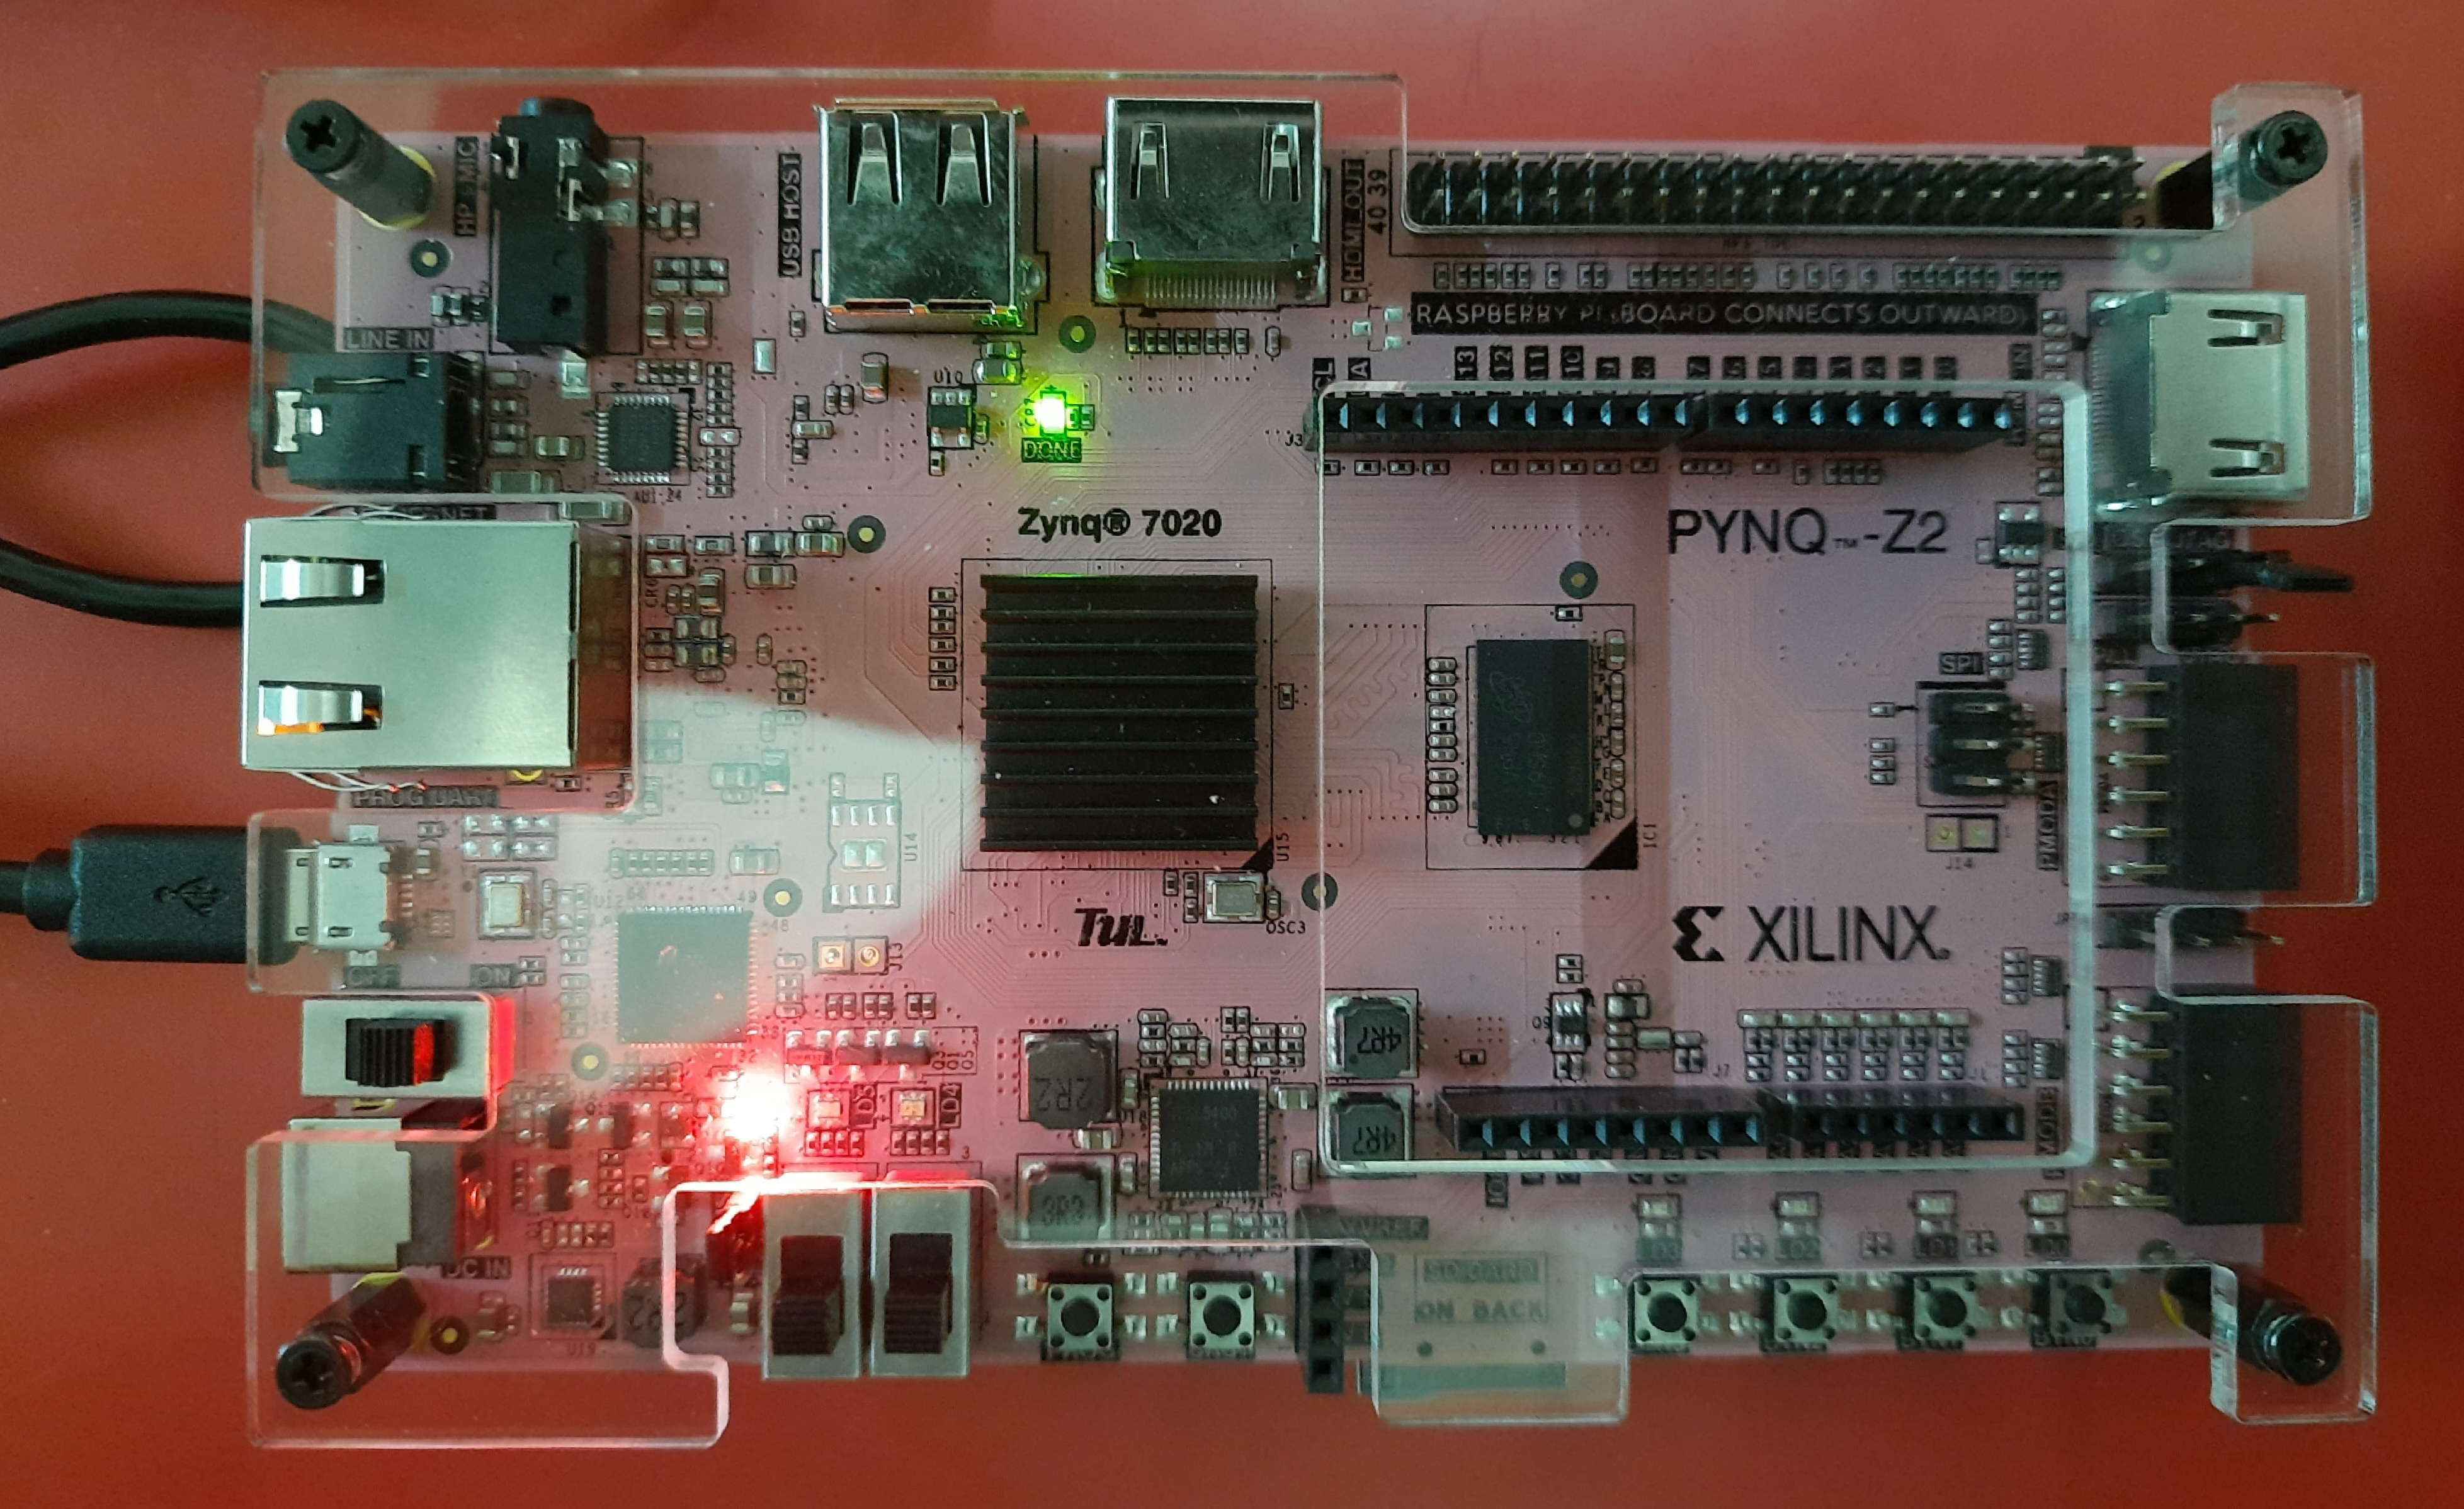
\includegraphics[width=1\linewidth]{images/expSetup.jpg}
        \caption{Experimental Setup}
        \label{fig:expSetup}
    \end{figure}

    \noindent
    A GUI based on Python's Tkinter library transfers the image to the FPGA. It also applies a grayscaling operation and an image resizing operation. Initially, a Serial port must be selected before beginning the image transfer. The figure \ref{fig:gui}  shows the designed GUI with some simple options such as Select Image, Transfer Image, About and EXIT. Also, before the image is transferred, it is shown on the screen.

    \begin{figure}[H]
        \centering
        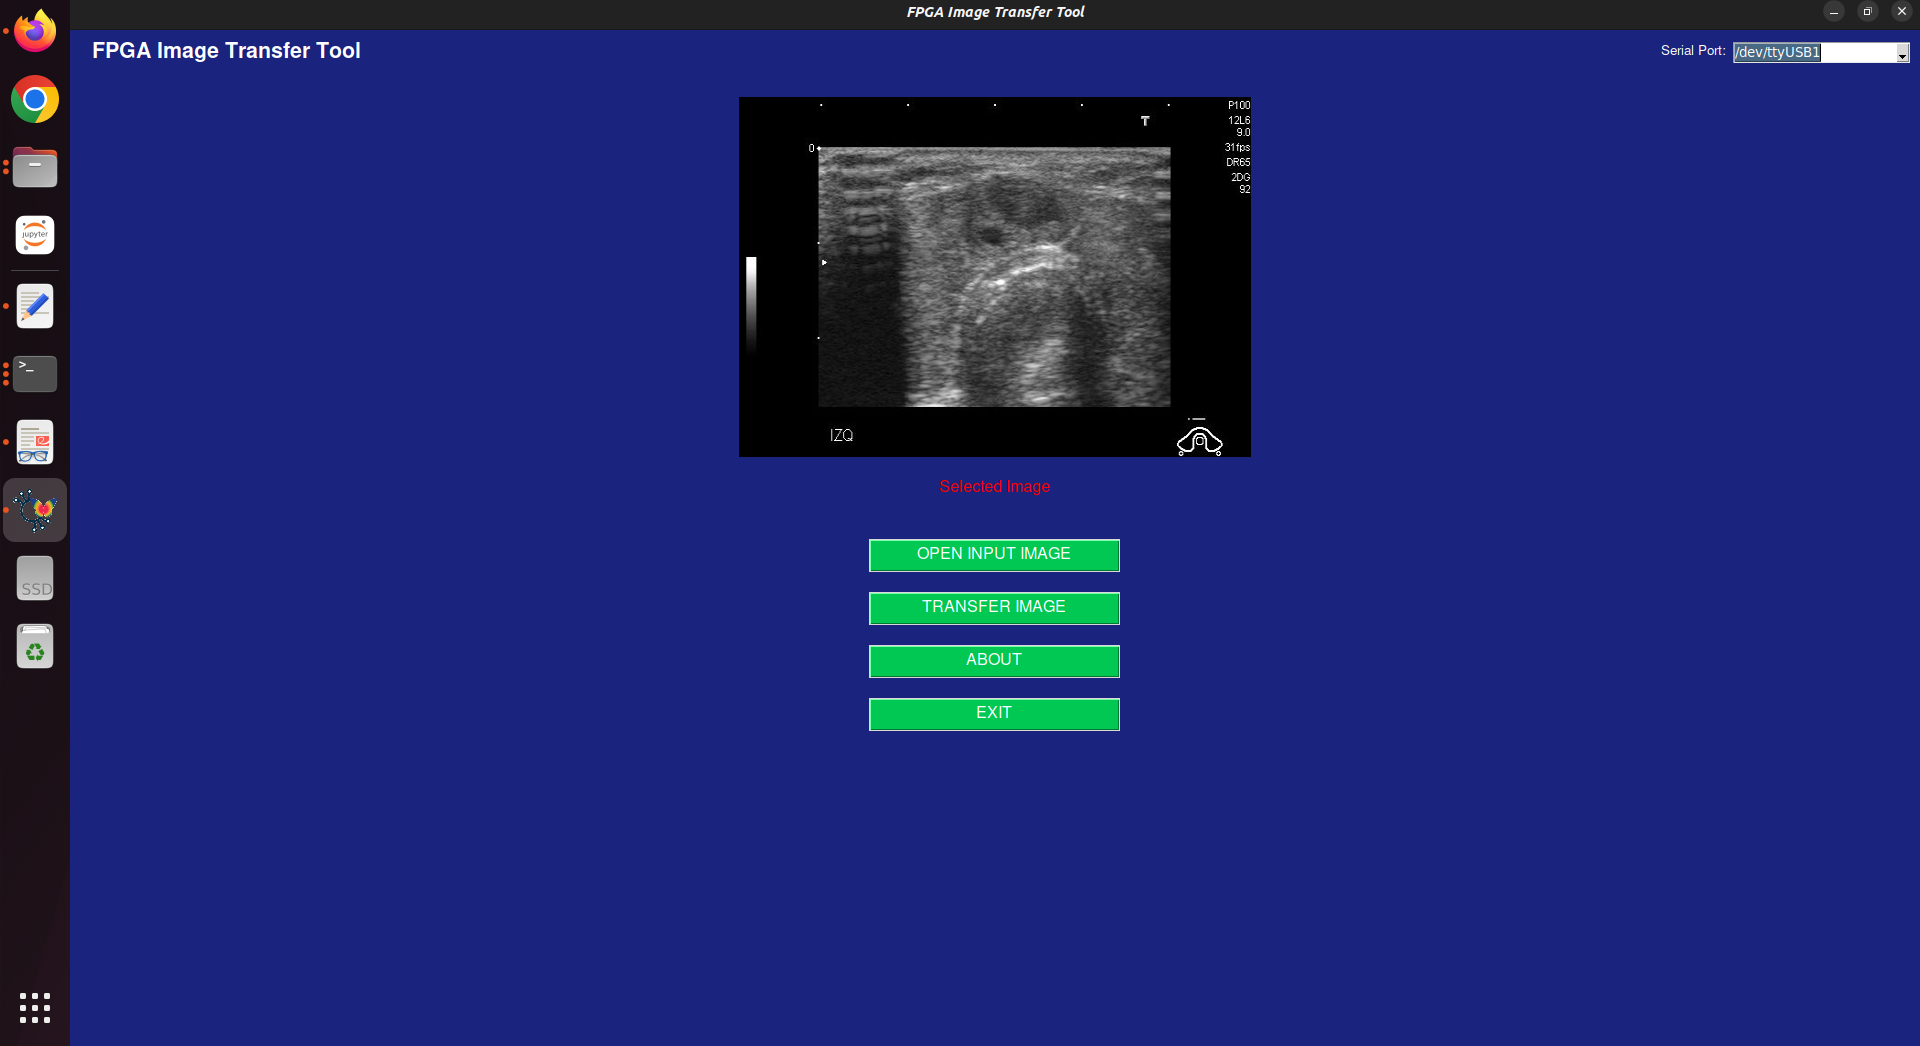
\includegraphics[width=1\linewidth]{images/gui.png}
        \caption{GUI for Image transfer to FPGA}
        \label{fig:gui}
    \end{figure}

    \noindent
    \textbf{Challenges \& Limitations}
    \par \noindent
    The CNN model is very complex, while designing the entire convolution and maxpool acceleration scheme, a lot of data dependencies need to be taken into account. Such a large design needs to be handled properly, ensuring proper architecture-level design since data dependencies need to be taken into account while designing all the compute and data logic. Another critical point is the fact that some of the rules which must be followed come up as a design limitation while designing. The resources and reference guide available for the use of the tools, specifically tutorials available, are very few being able to complete the entire design is a difficult task. The dataset in terms of the number of images available is quite a bit less in amount thus, the model is not that robust.

    

    


    

    

    
     


